\documentclass{article}
%------------PREAMBLE

\usepackage{stylesheet}
\usepackage{morefloats}
\setlength{\parindent}{12pt}

%---------------------------
                                          
\begin{document}

%---------------------------TITLE PAGE
\begin{titlepage}
\begin{center}

% Upper part of the page. The '~' is needed because \\
% only works if a paragraph has started.
\includegraphics[width=0.35\textwidth]{figures/uom_banner.pdf}~\\

% Title
\HRule \\[0.3cm]
{ \huge \bfseries Numerical Approaches to Quantum Chemistry - from Hückel Theory to the Hartree-Fock Approximation }\\

\HRule \\[0.8cm]

% Author and supervisor
\begin{minipage}{0.45\textwidth}
\begin{flushleft} \large
\textit{Author:}\\
\textit{Antonio Spataro}
\end{flushleft}
\end{minipage}
\begin{minipage}{0.45\textwidth}
\begin{flushright} \large
\textit{Subject Handbook code:}\\
\textit{COMP-90072}
\end{flushright}
\end{minipage}

\vspace{0.5cm}
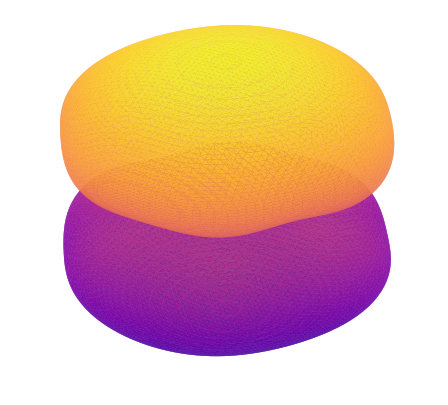
\includegraphics[width=0.50\textwidth]{figures/3d_pi.png}~\\[0.5cm]

% Place
{\large \textbf{The University of Melbourne}\\[0.2cm]
Faculty of Science - School of Physics}
\\[0.9cm]

% Submission date
{\large Date of Submission: 29th of May 2026}
\\[0.7cm]

% Lecturer
{\large Subject coordinators: Prof. Christian  Reichardt, A/Prof. Suzie Sheehy \& Prof. Harry Quiney}
\\
}

% Bottom of the page
\end{center}
\end{titlepage}

%---------------------------

%---------------------------TABLE OF CONTENTS
\tableofcontents
\pagebreak
%---------------------------

%---------------------------MAIN BODY
\section{Introduction}
\subsection{Report Outline}
This report has been broken up into 3 main sections:
\begin{enumerate}
    \item \textbf{Hückel Theory:}
    \begin{itemize}
        \item Ethylene and the Hückel Model
        \item Benzene - a more complicated molecule 
    \end{itemize}
    \item \textbf{The Hartree-Fock Approximation in the atomic regime:}
    \begin{itemize}
        \item Hydrogenic atoms
        \item General Atomic Hartree-Fock
    \end{itemize}
    \item \textbf{Molecular Hartree-Fock:}
    \begin{itemize}
        \item $H_2^+$
        \item Complex Molecules
    \end{itemize}
\end{enumerate}
\begin{figure}[h!]
    \centering
    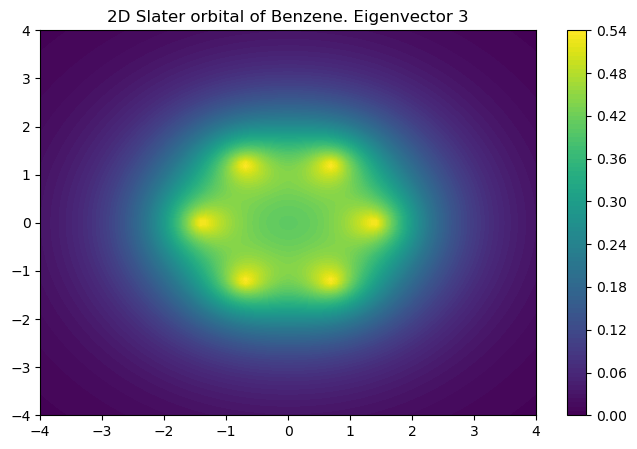
\includegraphics[width=0.7\linewidth]{figures/2D_Slater_Benzene_3.png}
    \caption{2D Slater Orbital of Benzene's 3rd Eigenvector}
\end{figure}
\subsection{Aim/Motivation:}
The fundamentals of quantum mechanics (QM) were first formulated separately by Max Planck, Albert Einstein and Niels Bohr from 1900 to 1913. The theory became more mathematically formal in the mid 1920's from the work of Bohr, Dirac, Heisenberg, Schrödinger and Born, as well as many other contributing physicists. With this increased formalism came the ability to describe atomic phenomena, and today QM is still the most accurate theory developed to describe physical processes on this scale. 
\\ \\
Quantum chemistry then uses QM techniques to observe the behaviour of both atoms, molecules and their respective interactions. It is the aim of this report to computationally investigate some of these techniques by:
\begin{itemize}
    \item Implementing code that allows us to plot 3D molecules
    \item Building a self-consistent field theory to solve for the ground state of various atoms and molecules
\end{itemize}

\pagebreak

\section{Theory}
\subsection{A brief overview on Quantum Mechanics}
\subsubsection{Wavefunctions and the Schr\"odinger Equation}
The most commonly understood formalism of QM uses wave mechanics through an object physicists call the \emph{wavefunction}, $\Psi(\vec{r},t)$. While a lot is still debated on the meaning of the wavefunction (Copenhagen vs many worlds vs other interpretations), for the purpose of this report, we can be satisfied by defining it as a description of a given quantum state. More accurately, it is a solution to the \emph{Schr\"odinger equation} (SE), given by:
\begin{equation}
    \hat{H} \Psi(\vec{r},t) = i\hbar \frac{\partial}{\partial t}\Psi(\vec{r},t)
    \label{eq1}
\end{equation}
Where $\hat{H}$ is the Hamiltonian operator \cite{sakurai2020modern}. More often then not, however, quantum chemistry uses what we call the \emph{time-independent Schr\"odinger equation} (TISE):
\begin{equation}
    \hat{H}\Psi(\vec{r}) = E\Psi(\vec{r})
    \label{eq2}
\end{equation}
This equation essentially tells us everything we need to know about a given system; a spatial wavefunction exists as an eigenvector of the Hamiltonian operator with energy eigenvalues, $E$. So, one can solve what is seemingly a simple eigenvalue problem, recover the wavefunction and then use further relatively simple techniques (such as the Born rule) to tell us everything we would like to know about a quantum system.
\\ \\ 
The problem is that even the TISE is often not exactly solvable as soon as we look beyond hydrogenic systems, thus we require new approximations and methodologies to allow us to describe complicated atoms and molecules. 

\subsubsection{The Born-Oppenheimer Approximation}
Most of what follows in the report directly relies on one key approximation; that being the one made by Born and Oppenheimer in 1927 \cite{Born1927}, stating that nuclear positions are fixed relative to rapidly moving electrons such that said electrons occupy states which are solutions to \cref{eq2}. Thus, the Born-Oppenheimer approximation (BOA) is one that represents an adiabatic model of molecules, which they justified due to the fact that the mass of any given nucleus is orders of magnitudes larger than that of a system of electrons ($m_e = 0.0005486 \ au$). 

For a molecular system, the wavefunction we have depends on both the nuclear position, $\vec{R}_N$, and electron position, $\vec{r}_e$, meaning we can write $\Psi(\vec{r}_e, \vec{R}_N)$. The Hamiltonian operator in the TISE must also contain these position operator and, under the BOA, we can write the total Hamiltonian of a molecular system as:
\begin{equation}
    H_{total} = H_{electron}+H_{nucleus} = (T_e + V_{ee} + V_{eN}) + (T_N + V_{NN})
    \label{eq3}
\end{equation}
Thus we can separate the TISE into two separate eigenvalue problems, one solving for the electron eigenfunction, $\psi_i(\vec{r}_e,\vec{R}_N)$, and its associated eigen-energies $U_i(\vec{R}_N)$, and the other solving for the nuclear wavefunction $\Phi_i(\vec{R}_N)$ and energies $E_i$. This is clearly already getting very complicated, hence the need for approximation methods which are the focus of this report.
\subsection{Computational Approximation Methods}
\subsubsection{The H\"uckel Molecular Orbital Approximation}




\pagebreak
\section{Bibliography}
\nocite{*} 
\bibliographystyle{unsrt}
\bibliography{biblio}


\end{document}